\documentclass[11pt]{article}
\usepackage{geometry}                % See geometry.pdf to learn the layout options. There are lots.
\geometry{letterpaper}                   % ... or a4paper or a5paper or ... 
%\geometry{landscape}                % Activate for for rotated page geometry
%\usepackage[parfill]{parskip}    % Activate to begin paragraphs with an empty line rather than an indent
\usepackage{graphicx}
\usepackage{amssymb}
\usepackage{epstopdf}
\usepackage{amsmath}
\DeclareGraphicsRule{.tif}{png}{.png}{`convert #1 `dirname #1`/`basename #1 .tif`.png}

\title{Mathematical representation of the drought decision model - Shiny Version}
\author{Trisha Shrum}
%\date{}                                           % Activate to display a given date or no date

\begin{document}
\maketitle
%\section{}
%\subsection{}

\section{Model}

The goal of the player is to maximize the following objective function:

\begin{equation}
\sum_{t=1}^T \pi_t(1+r)^{-t}
\end{equation}

subject to the following constraints:

\section{Scripts}

\subsection{global.R}
\begin{enumerate}
\item Sources other scripts
\item Javascript coding
\item Populate a new environment with rainfall gauge info: \verb!getStationGauge()!
\item Populate a new environment with constant (user) variables: \verb!getConstantVars()!
\item Setting additional variables: acres, start years, simulation lengths
\item Create state variables for practice and full runs: \verb!getSimVars()!
\item Create lists of variables for practice and full runs: \verb!practiceRuns!, \verb!simRuns!
\item Establish additional settings
\end{enumerate}  
 
\subsection{load.R}
Loads necessary packages

\subsection{shinySupportFunctions.R}
\begin{enumerate}
\item \verb!getJulyInfo! function: Calculates available and predicted forage in July, creates a
    UI to display info and allows user to select adaptation level.
    \begin{itemize}
    \item Called in \verb!simUI.R!
    \end{itemize}
\item \verb!getCowSell! function: Creates a UI for the user to select how many cows and calves to sell. Called in \verb!simUI.R!.
\item \verb!shinyInsurance! function: Calculates premium and indemnification for a specific year and grid cell. Currently, returns are summed but this could be done on a index interval basis instead.
\end{enumerate}

\subsection{forageFunctions.R}

\begin{itemize}
	\item \verb!getForagePotential! function: Returns an index representing
  annual forage production for a given gridcell or station gauge's annual precipitation record. Called in \verb!calfCowFunctions.R!.
	\item \verb!whatIfForage! function: calculates expected forage for a given scenario. Called in \verb!shinySupportFunctions.R! and \verb!simUI.R!.
	\item \verb!getMLRAWeights! function: Computes forage potential weights using the
  mean of plant growth curves by MRLA for a specified state. Called in \verb!initialFunctions.R!.
  	\item \verb!COOP_in_MLRA! function: Returns the MLRA in which a specified
  coop site is located. Called in \verb!initialFunctions.R!.
\end{itemize}

\subsection{adaptationFunctions.R}

\begin{itemize}
	\item \verb!calculateAdaptationIntensity! function: Takes forage potential and an adaptation intensity factor to provide a scalar of drought action. If forage potential is above 1 (no drought), then this variable goes to 0 (no adaptation). Called in \verb!shinySupportFunctions.R! and \verb!simUI.R!.
\end{itemize}

\subsection{costRevenueFunctions.R}

\begin{itemize}
	\item \verb!calculateExpSales! function: Calculates expected calf revenues for non-drought year. 
	\item \verb!calculateFeedCost! function: Calculates the costs of purchasing additional feed. Called in \verb!getAdaptCost! in \verb!costRevenueFunctions.R!. 
	\item \verb!CalculateRentPastCost! function: Calculates the costs of renting pasture and trucking pairs. Called in \verb!getAdaptCost! in \verb!costRevenueFunctions.R!.
	\item \verb!getAdaptCost! function: Calculates the cost of adaptation based on strategy, intensity needed, days, and herd size. Called in \verb!shinySupportFunctions.R! and \verb!simUI.R!.
\end{itemize}

\subsection{initialFunctions.R}

\begin{itemize}
	\item \verb!getConstantVars! function: Reads in constant variables into a
  \verb!constvars! environment using the  file \verb!data/constant_vars.csv!. Called in \verb!global.R!.
  	\item \verb!getSimVars! function: Creates list of simulation variables. Called in \verb!global.R!.
  	\item \verb!getStationGauge! function: Returns precipitation record and locational attributes for the target location. Default is Central Plains Experimental Range (CPER) but alternative locations at COOP sites across Colorado may be specified. Called in \verb!global.R!.
  	\item \verb!createResultsFrame! function: This function creates a theoretical previous result from the year before the simulation begins right now this assumes that there was no drought the year before the simulation and revenues were 0. These assumptions are likely unrealistic and can be adjusted to accomodate different scenarios. Called in \verb!shinySupportFunctions.R! and \verb!server.R!.
\end{itemize}

\subsection{calfCowFunctions.R}

\begin{itemize}
	\item \verb!AdjWeanSuccess! function: Adusts weaning success downward for the year of the drought and the following year. Called in \verb!simUI.R!.
	\item \verb!calfDroughtWeight! function: If forage potential is less than 1, then the calf weight is less than the optimal weight. Called in \verb!shinySupportFunctions.R! and \verb!simUI.R!.
	\item \verb!calfWeanWeight! function: Computes calf weights based on station/grid cell forage potential for a n-year period. Called in \verb!initialFunctions.R!.
	\item \verb!shinyHerd! function: calculates the size of herd for the shiny app. Called in \verb!simUI.R!.
\end{itemize}

\subsection{assetFunctions.R}
\begin{itemize}
	\item \verb!CalcCowAssets! function: Calculates the cow assets for each year. Called in \verb!initialFunctions!.
\end{itemize}


\section{Function Details}
Key functions in the model are listed and described in alphabetical order.


\subsection{AdjWeanSuccess}
\begin{itemize}
\item Function: \verb!AdjWeanSuccess!
	\begin{itemize}
	\item Description: Adjusts weaning success downward for the year of the drought and the following year. If forage production falls below 1 in year $t=1$, then weaning percentage falls slightly in year $t=1$ and more drastically in year $t=2$. If forage production falls below 1 in a year $t=1$ where weaning percentage was already decremented because of previous forage production deficits or insufficient culling, then weaning percentage falls further in years $t=1,2$ than it would have if the starting point was at the maximum weaning percentage.
	\item Inputs: \verb!totalForage!, \verb!totalForage1ya!, \verb!normal.wn.succ!
	\item Output: \verb!wn.succ!
	\item Assumptions: This equation is based on what I consider to be ``reasonable" estimates of weaning success based on forage potential. These fall roughly in line with body condition scores from the \textit{Nutrient Requirements of Beef Cattle}, but are only ballpark estimates.
	\end{itemize}
\end{itemize}

The weaning percentage maximum is 88\%, represented by $\tilde{\omega}$. Weaning percentage in year $t$, $\omega_t$, is given by:\\

\begin{equation}
\omega_t =
\begin{cases}
\tilde{\omega}  &\text{if } F_{t}, F_{t-1} \ge 1  \\
\tilde{\omega} * F_{t}^{(1/4)} &\text{if } F_{t} < 1 \land F_{t-1} \ge 1 \\
\tilde{\omega} * F_{t - 1} &\text{if } F_{t} \ge 1 \land F_{t-1} < 1 \\
\tilde{\omega} * F_{t}^{(1/4)} * F_{t-1} &\text{if } F_{t}, F_{t-1} < 1 \\
\end{cases}
\end{equation}

\vspace{.25in}
\textbf{Code:}

\verb!  wn.succ <- NULL!

\verb!  if(totalForage < 1 & totalForage1ya >= 1){!

\verb!    wn.succ <- normal.wn.succ * totalForage^.25!

\verb!  }else if(totalForage >= 1 & totalForage1ya < 1){!

\verb!    wn.succ <- normal.wn.succ * totalForage1ya!

\verb!  }else if(totalForage < 1 & totalForage1ya < 1){!

\verb!    wn.succ <- normal.wn.succ * totalForage1ya * totalForage^.25!

\verb!  }else if(totalForage >= 1 & totalForage1ya >= 1){!

\verb!    wn.succ <- normal.wn.succ!

\verb!  }!





\subsection{getStationGauge}
The model is currently set for a default to the Central Plans Experimental Range (CPER), but alternative locations for COOP sites in Colorado may also be used.

\begin{itemize}
\item Function: \verb!getStationGauge!
	\begin{itemize}
	\item Description: Returns precipitation record and locational attributes for the target
  location. Default is Central Plains Experimental Range (CPER).
  \item Inputs: \verb!target.loc! (target location. default set to \verb!CPER!)
  \item Outputs: a list called \verb!station.gauge! that contains \verb!monthlyPrecipWeights! (the weight given to precipitation in each month in terms of how much it contributes to annual forage), \verb!precip! (station or gauge precipitation data from 1948 to 2015), \verb!gridCell! (Target Grid Cell for reading in PRF index values at a given point in time).
	\end{itemize}
\end{itemize}

\textbf{If CPER (default):}
\begin{enumerate}
\item Monthly precipitation weights are based on the plant growth curves for rangeland with loamy soils in major land resource area 67B (see Figure \ref{MLRA}, an area that encompasses a large portion of Eastern Colorado including the CPER site (Site ID: R067BY002CO). We use the plant growth curve for Western Wheatgrass, Blue Grama, Green Needlegrass, Fourwing Saltbush Plant Community (Growth curve number CO6701), which is well suited for grazing and is maintained with properly stocked prescribed grazing. 

\begin{figure}
\begin{center}
\label{MLRA}
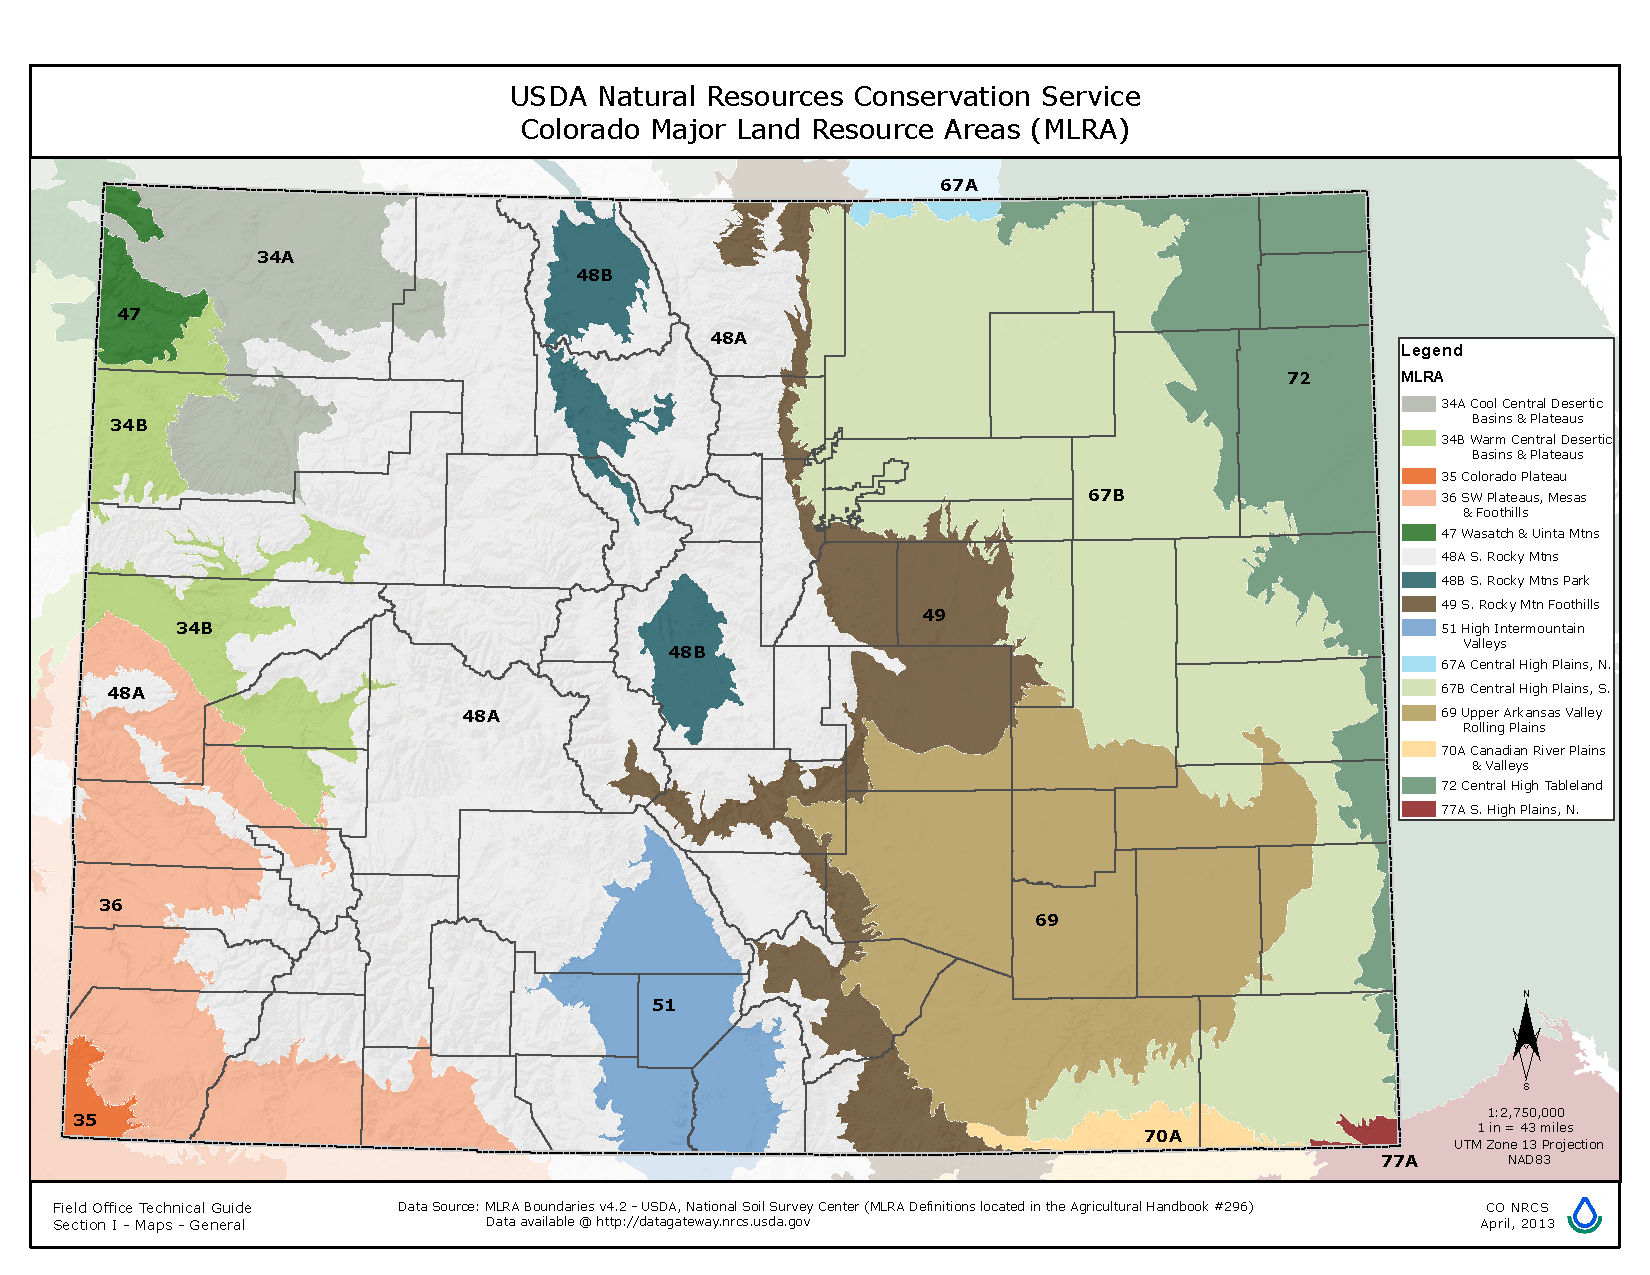
\includegraphics[scale=.5]{CO_MLRAs}
\end{center}
\caption{Major Land Resource Areas for Colorado}
\end{figure}

These monthly weights are the percentage of plant growth that is expected in each month during a normal year. Under normal conditions, total annual production averages 1300 pounds per acre. These weights add up to 1. 

\begin{tabular}{|cccccccccccc|}
\hline
Jan & Feb & Mar & Apr &May & Jun & Jul & Aug &Sep & Oct& Nov& Dec \\
\hline
0  & 0 &0.02& 0.08 &0.2 &0.28 &0.15 &0.12 &0.1 &0.05 &  0 &  0 \\
\hline
\end{tabular}

\item Station Gauge, historical precipitation totals dating back to 1948, which are also read in from the Excel model. Precip totals are collected at CPER itself and do not rely on precip data from COOP sites.
\item The target grid cell 25002 is assigned to the PRF grid cell (assuming this is the correct grid cell)
\end{enumerate}


\section{Default Model Values}

\begin{itemize}
\item Starting herd size: 600 cows
\item Ranch size: 3000 acres
\item Carrying capacity: 5 acres/cow
\item Maximum calf weaning weight: 600 lbs
\item Default calf sale rate: 75\%
\item Maximum weaning percentage: 88\%
\item Cow price: \$850/cow
\item Calf price at weaning: \$1.40/pound
\item Cow mortality rate: 4\%
\item Practice round years: 1951-1955
\item Game round years: 1999-2008
\item Household expenses: \$60,000
\item Starting cash assets: \$90,000
\item Operating costs: \$500/cow
\item Insurance Coverage Level: 90\%
\item Interest rate: 5\%
\end{itemize}



  


 \end{document}